\documentclass{article}
\usepackage{fullpage}
\usepackage{enumitem}
\usepackage{verbatim}
\usepackage{tikz}
\usetikzlibrary{trees}
\begin{document}
\title{CMSI 386 Homework \#4}
\author{Zane Kansil \& Edward Bramanti}
\maketitle
\begin{enumerate}
    \item Write Regular Expressions for: 
    \begin{enumerate}
        \item Canadian Postal Codes:
        \begin{verbatim}
        [^DFIOQUWZ][\d][^DFIOQU] [\d][^DFIOQU][\d]
        \end{verbatim}
        \item Legal Visa® Card Numbers, not including checksums
        \begin{verbatim}
        4\d{3} (\d{4} ){3}
        \end{verbatim}
        \item MasterCard® Numbers, not including checksums
        \begin{verbatim}
        5\d{3} (\d{4} ){3}
        \end{verbatim}
        \item Ada 95 numeric literals
        \begin{verbatim}
        \d(_?\d)*#[\dA-F](_?[\dA-F])*#(E[+-]+[\dA-F](_?[\dA-F])*)?|\d(_?\d)*(\.\d(_?\d)*)?(E[+-]+\d(_?\d)*)?
        \end{verbatim}
        \item Strings of letters and numbers beginning with a letter, EXCEPT those strings that are exactly three letters ending with two Latin letter ohs, of any case.
        \begin{verbatim}
        ^\w(?![Oo][Oo]$)[\w\d]*
        \end{verbatim}
    \end{enumerate}
    \pagebreak
    \item Syntax tree for Program in JSON (http://cs.lmu.edu/~ray/notes/syntax/)
    \verbatiminput{syntax-tree.js}
    \pagebreak
    \item In the Ada language comments are started with "--" and go to the end of the line. Therefore the designers decided not to make the unary negation operator have the highest precedence. Explain why this choice was made. Also, give an abstract syntax tree for the expression -8 * 5 and explain how this is similar to and how it is different from the alternative of dropping the negation from EXP2 and adding - EXP5 to EXP4. \\
    The designers made this choice so that you can have a \texttt{NEG|POS - POS} or a \texttt{NEG|POS + POS}, but never a \texttt{NEG|POS ± NEG}. Essentially, only positive numbers can be the second parameter of a binary addition. If someone were to do \texttt{9--5} today, many programs have syntax highlighting which would alert the programmer to their code being commented out. Nevertheless, when Ada was designed, syntax highlighting may not have been as advanced; therefore, it was necessary for the laguage designers to carefully consider what to do with this programming conflict. \\
    TIKS GOES HERE \\
    RATIONALE GOES HERE \\
    \pagebreak
    \item Here is a description of a language. Programs in this ``language'' are made up of a non-empty sequence of function declarations, followed by a single expression. Each function declaration starts with the keyword fun followed by the function's name (an identifier), then a parenthesized list of zero or more parameters (also identifiers) separated by commas, then the body, which is a sequence of one or more expressions terminated by semicolons with the sequence enclosed in curly braces. Expressions can be numeric literals, string literals, identifiers, function calls, or can be made up of other expressions with the usual binary arithmetic operators (plus, minus, times, divide) and a unary prefix negation and a unary postfix factorial (``!''). There's a conditional expression with the weird syntax \texttt{"x if y else z"}. Factorial has the highest precedence, followed by negation, the multiplicative operators, the additive operators, and finally the conditional. Parentheses are used, as in most other languages, to group subexpressions. Numeric literals are non-empty sequences of decimal digits with an optional fractional part and an optional exponent part. 
    String literals are delimited with double quotes with escape sequences followed by four hexadecimal digits. Identifiers are non-empty sequences of letters, decimal digits, underscores, at-signs, and dollar signs, beginning with a letter or dollar sign, that are not also reserved words. Function calls are formed with an identifier followed by a comma-separated list of expressions bracketed by parentheses. There are no comments in this language, and whitespace can be used liberally between tokens.
    Write the micro and macrosyntax of this language.
    \verbatiminput{macro-syntax-question.txt}
    \pagebreak
    \item Give an abstract syntax tree for the following Java code fragment:
    \begin{verbatim}
    if (x > 2 || !String.matches(f(x))) {
        write(- 3*q);
    } else if (! here || there) {
        do {
            while (close) tryHarder();
            x = x >>> 3 & 2 * x;
        } while (false);
        q[4].g(6) = person.list[2];
    } else {
        throw up;
    }
    \end{verbatim}
    \begin{center}
    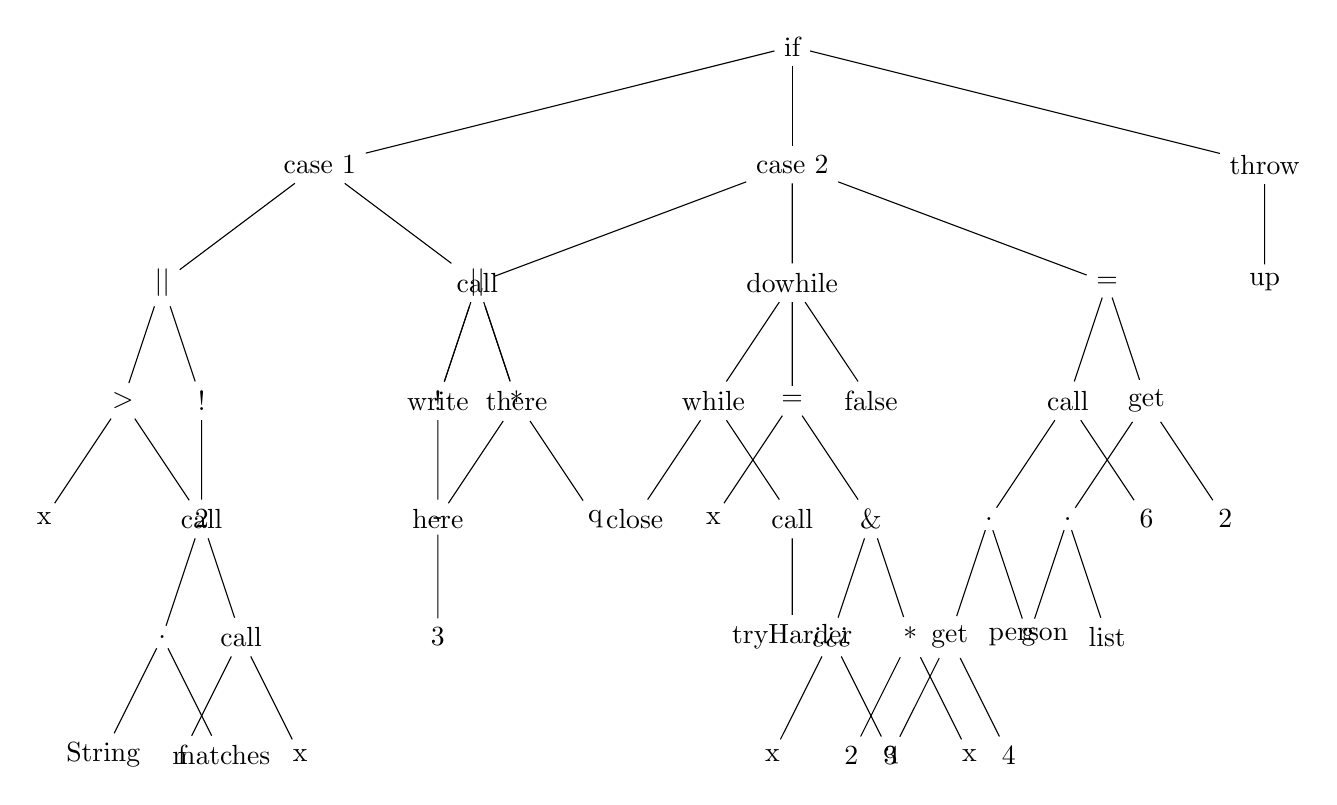
\begin{tikzpicture}[level distance=1.5cm,
      level 1/.style={sibling distance=6cm},
      level 2/.style={sibling distance=4cm},
      level 3/.style={sibling distance=1cm},
      level 4/.style={sibling distance=2cm},
      level 5/.style={sibling distance=1cm},
      level 6/.style={sibling distance=1.5cm},
      level 7/.style={sibling distance=1.5cm}
    ]
    \node {if}
        child {node{case 1}
            child {node{\(\vert\)\(\vert\)}
                child {node{\textgreater}
                    child {node{x}}
                    child {node{2}}
                }
                child {node{!}
                    child {node{call}
                        child {node{.}
                            child {node{String}}
                            child {node{matches}}
                        }
                        child {node{call}
                            child {node{f}}
                            child {node{x}}
                        }
                    }
                }
            }
            child {node{call}
                child {node{write}}
                child {node{*}
                    child {node{-}
                        child {node{3}}
                    }
                    child {node{q}}
                }
            }
        }
        child {node{case 2}
            child {node{\(\vert\)\(\vert\)}
                child {node{!}
                    child {node{here}}
                }
                child {node{there}}
            }
            child {node{dowhile}
                child {node{while}
                    child {node{close}}
                    child {node{call}
                        child{node{tryHarder}}
                    }
                }
                child {node{=}
                    child {node{x}}
                    child {node{\&}
                        child {node{>>>}
                            child {node{x}}
                            child {node{3}}
                        }
                        child {node{*}
                            child {node{2}}
                            child {node{x}}
                        }
                    }
                }
                child {node{false}}
            }
            child {node{=}
                child {node{call}
                    child {node{.}
                        child {node{get}
                            child {node{q}}
                            child {node{4}}
                        }
                        child {node{g}}
                    }
                    child{node{6}}
                }
                child {node{get}
                    child {node{.}
                        child {node{person}}
                        child {node{list}}
                    }
                    child {node{2}}
                }
            }
        }
        child {node{throw}
            child {node{up}}
        };
    \end{tikzpicture}
    \end{center}
\end{enumerate}
\end{document}
